\chapter[Evaluation of the ADP-GDA metric]{Performance of the ADP-GDA metric on constrained clustering benchmarks}
\label{apx:adsmetric}

\section*{Introduction}

We have proposed a novel approach for learning a metric for clustering with pairwise constraints in Section 2.5.2 and have used it to model human spatial representation structure in Chapter 5, showing that it can help predict whether buildings are co-represented (belong to the same sub-map in spatial memory) in a large majority of cases. Here, we briefly summarize the difference of this approach from other metric learning methods, and present some preliminary results of its performance compared to state of the art approaches.

The framework using a generative classifier as a distance function can be seen as a novel approach to perform non-linear metric learning using weak supervision in the form of pairwise constraints, in order to improve clustering performance, as pioneered in its linear form by \citep{xing2002distance}. Although this problem is very similar to metric learning in general, the criterion of interest is often somewhat different: as opposed to optimizing the performance of some classifier as in e.g. \citep{bellet2012similarity}), or for a large margin as in e.g. \citep{weinberger2005distance}, the goal is ensuring that all instances of a cluster are closer under the learned metric than those of different clusters. 

For general applicability, non-linear metrics are vital, because of the problem of \textit{multimodality}. When data points forming several groups or `modes' in unweighted feature space actually belong to the same cluster semantically, as indicated by ML constraints, there exists no linear projection able to separate them, and linear methods must inevitably fail. A traditional example is the XOR dataset, consisting of four groups, connected by diagonal ML constraints, such that there exists no linear separating hyperplane - see Figure \ref{fig:motivation2}a. 

Although kernel-based methods can deal with multimodal clustering problems (or any complicated data distribution) according to the Representer Theorem, in theory, given the optimal kernel and suitable parameters, in practice it is often difficult to find such a kernel. Most non-linear metric learning methods able to learn suitable kernels are sensitive to multiple hyperparameters, and, being nonconvex optimization problems, frequently get stuck in local minima.

A further issue with popular isotropic kernels such as the Radial Basis Function (RBF), frequently used in non-linear metric learning \citep{baghshah2010kernel, chitta2011approximate}, is that they are ill-suited for data with features on very different scales, since the optimal regularization parameters in one dimension can be suboptimal in other dimensions in this case, as pointed out by \citep{ong2005learning} (who propose a solution only in the supervised setting). 

\begin{figure*}[t]
	\centering
	
	\subfloat[XOR dataset]{%
		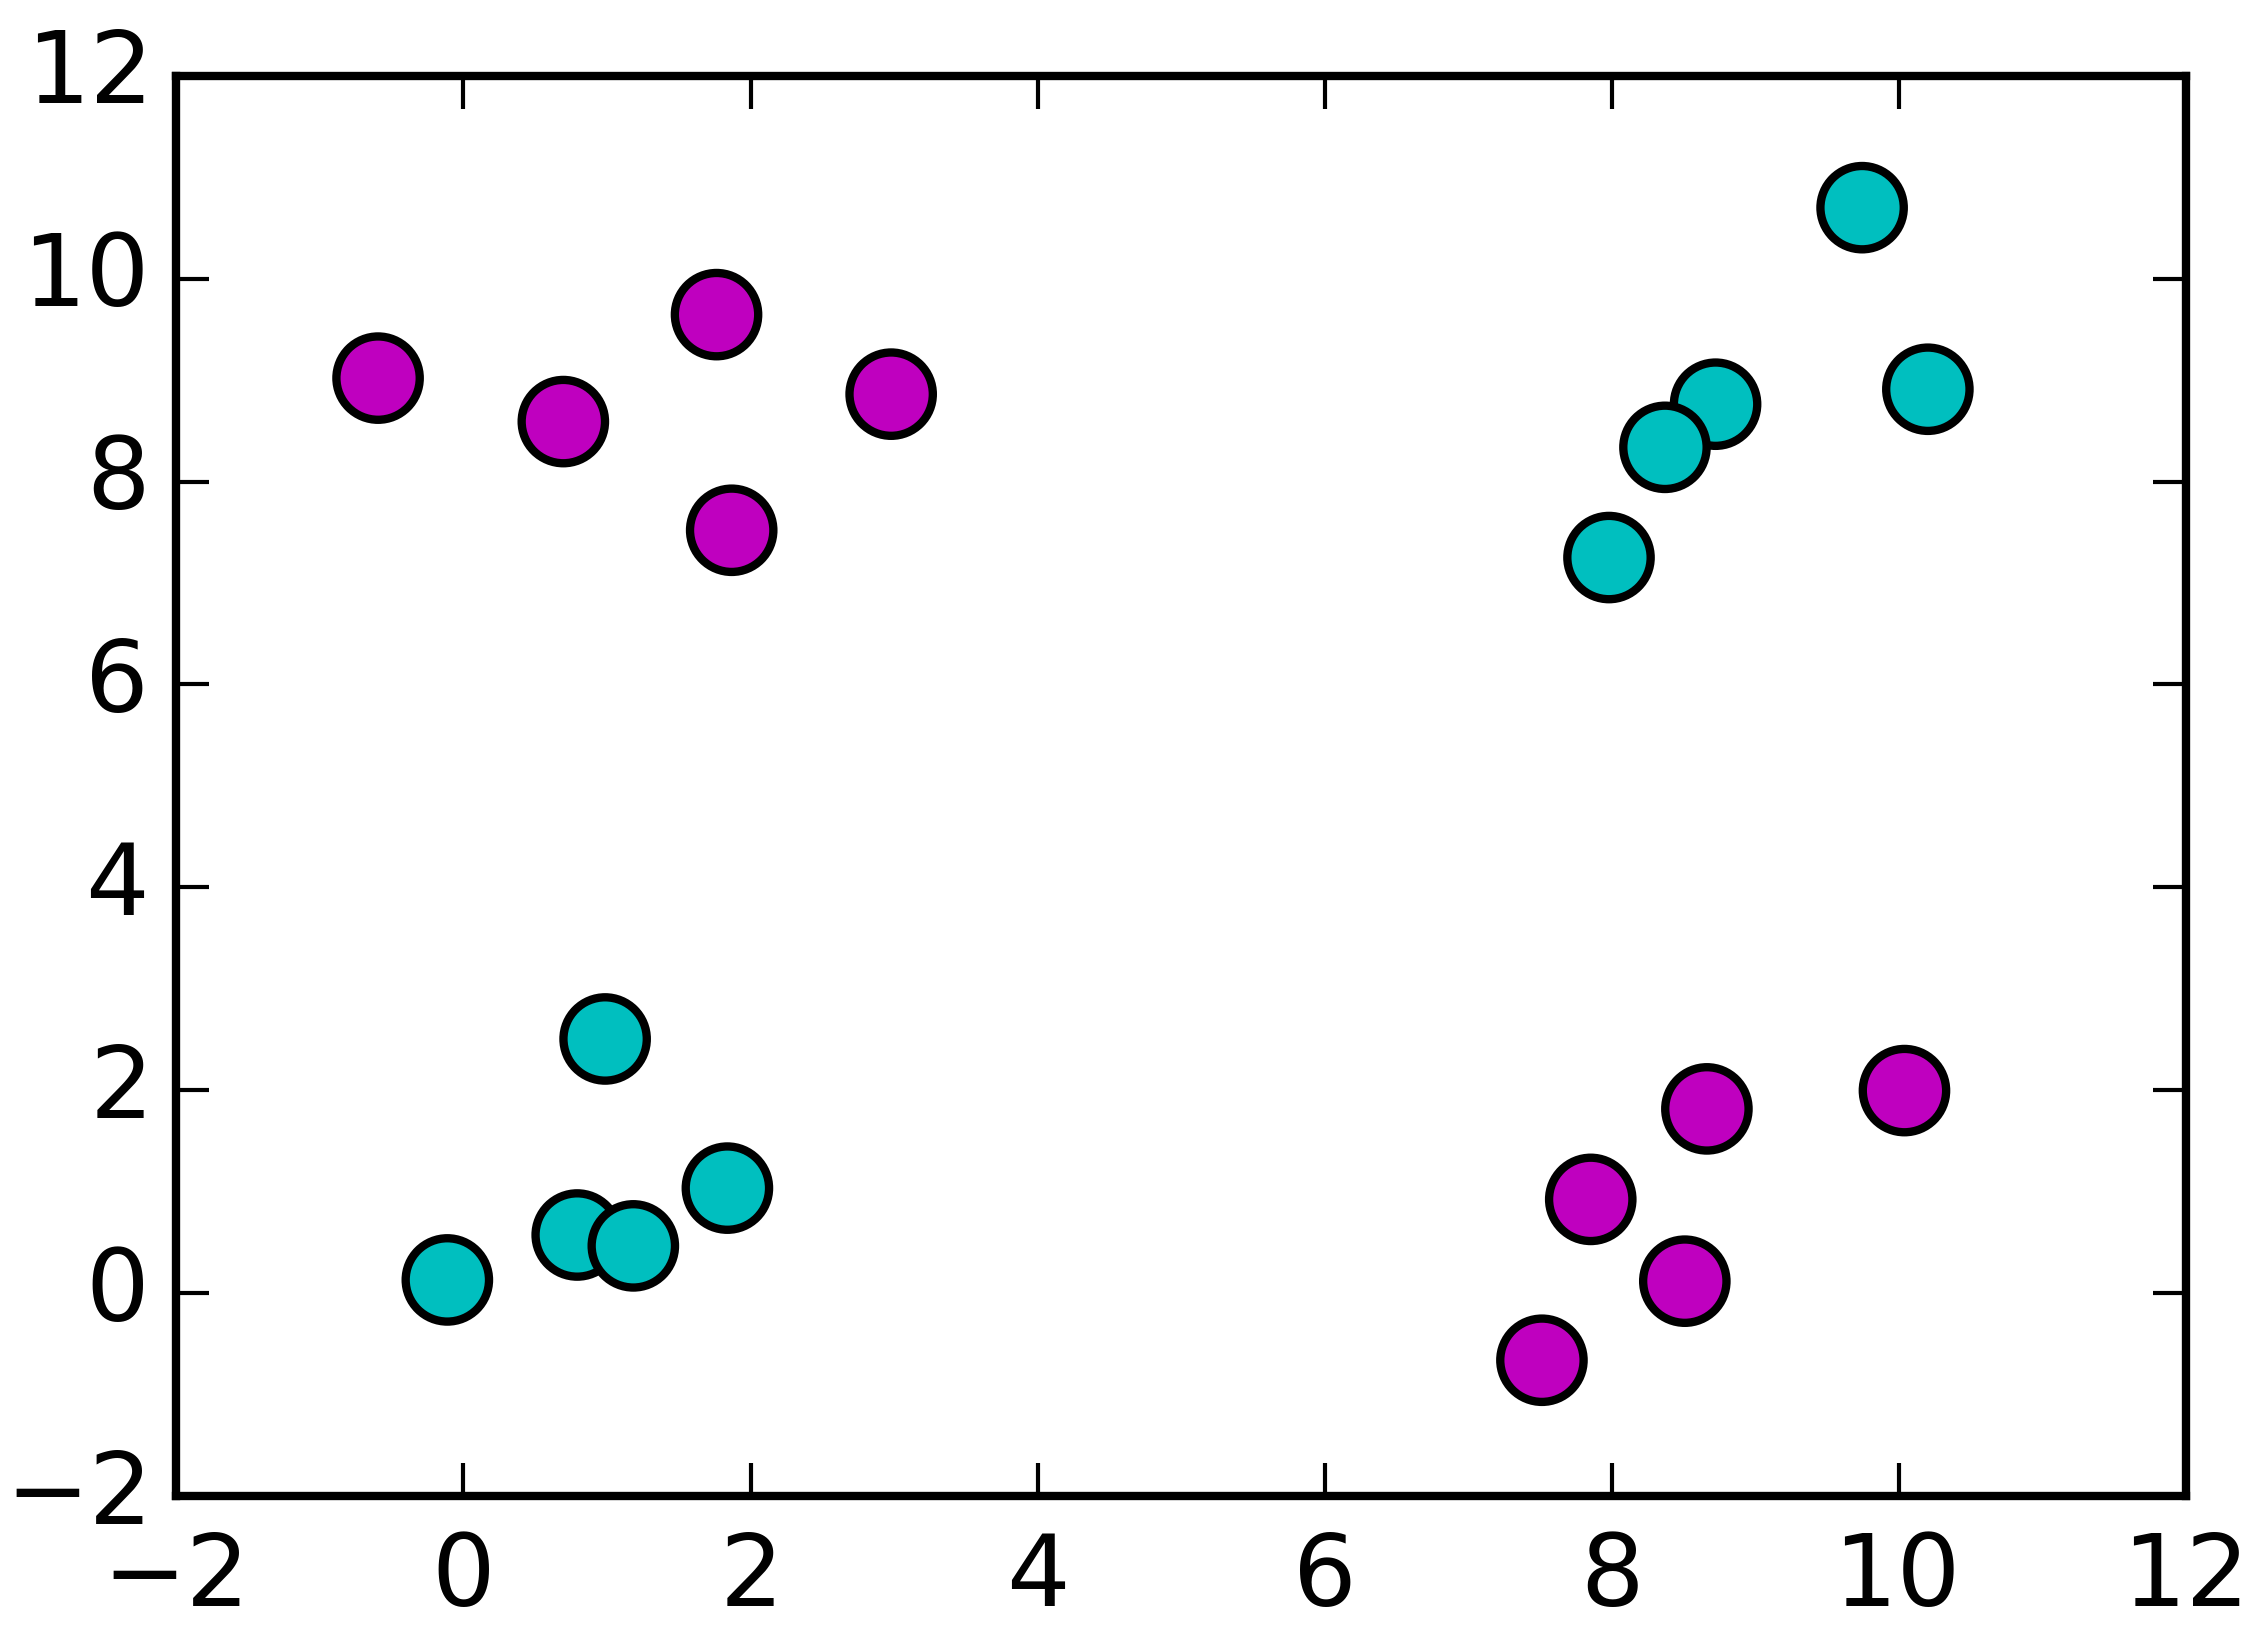
\includegraphics[width=0.25\textwidth]{quadplot1}%
	}
	\subfloat[Pairwise differences]{%
		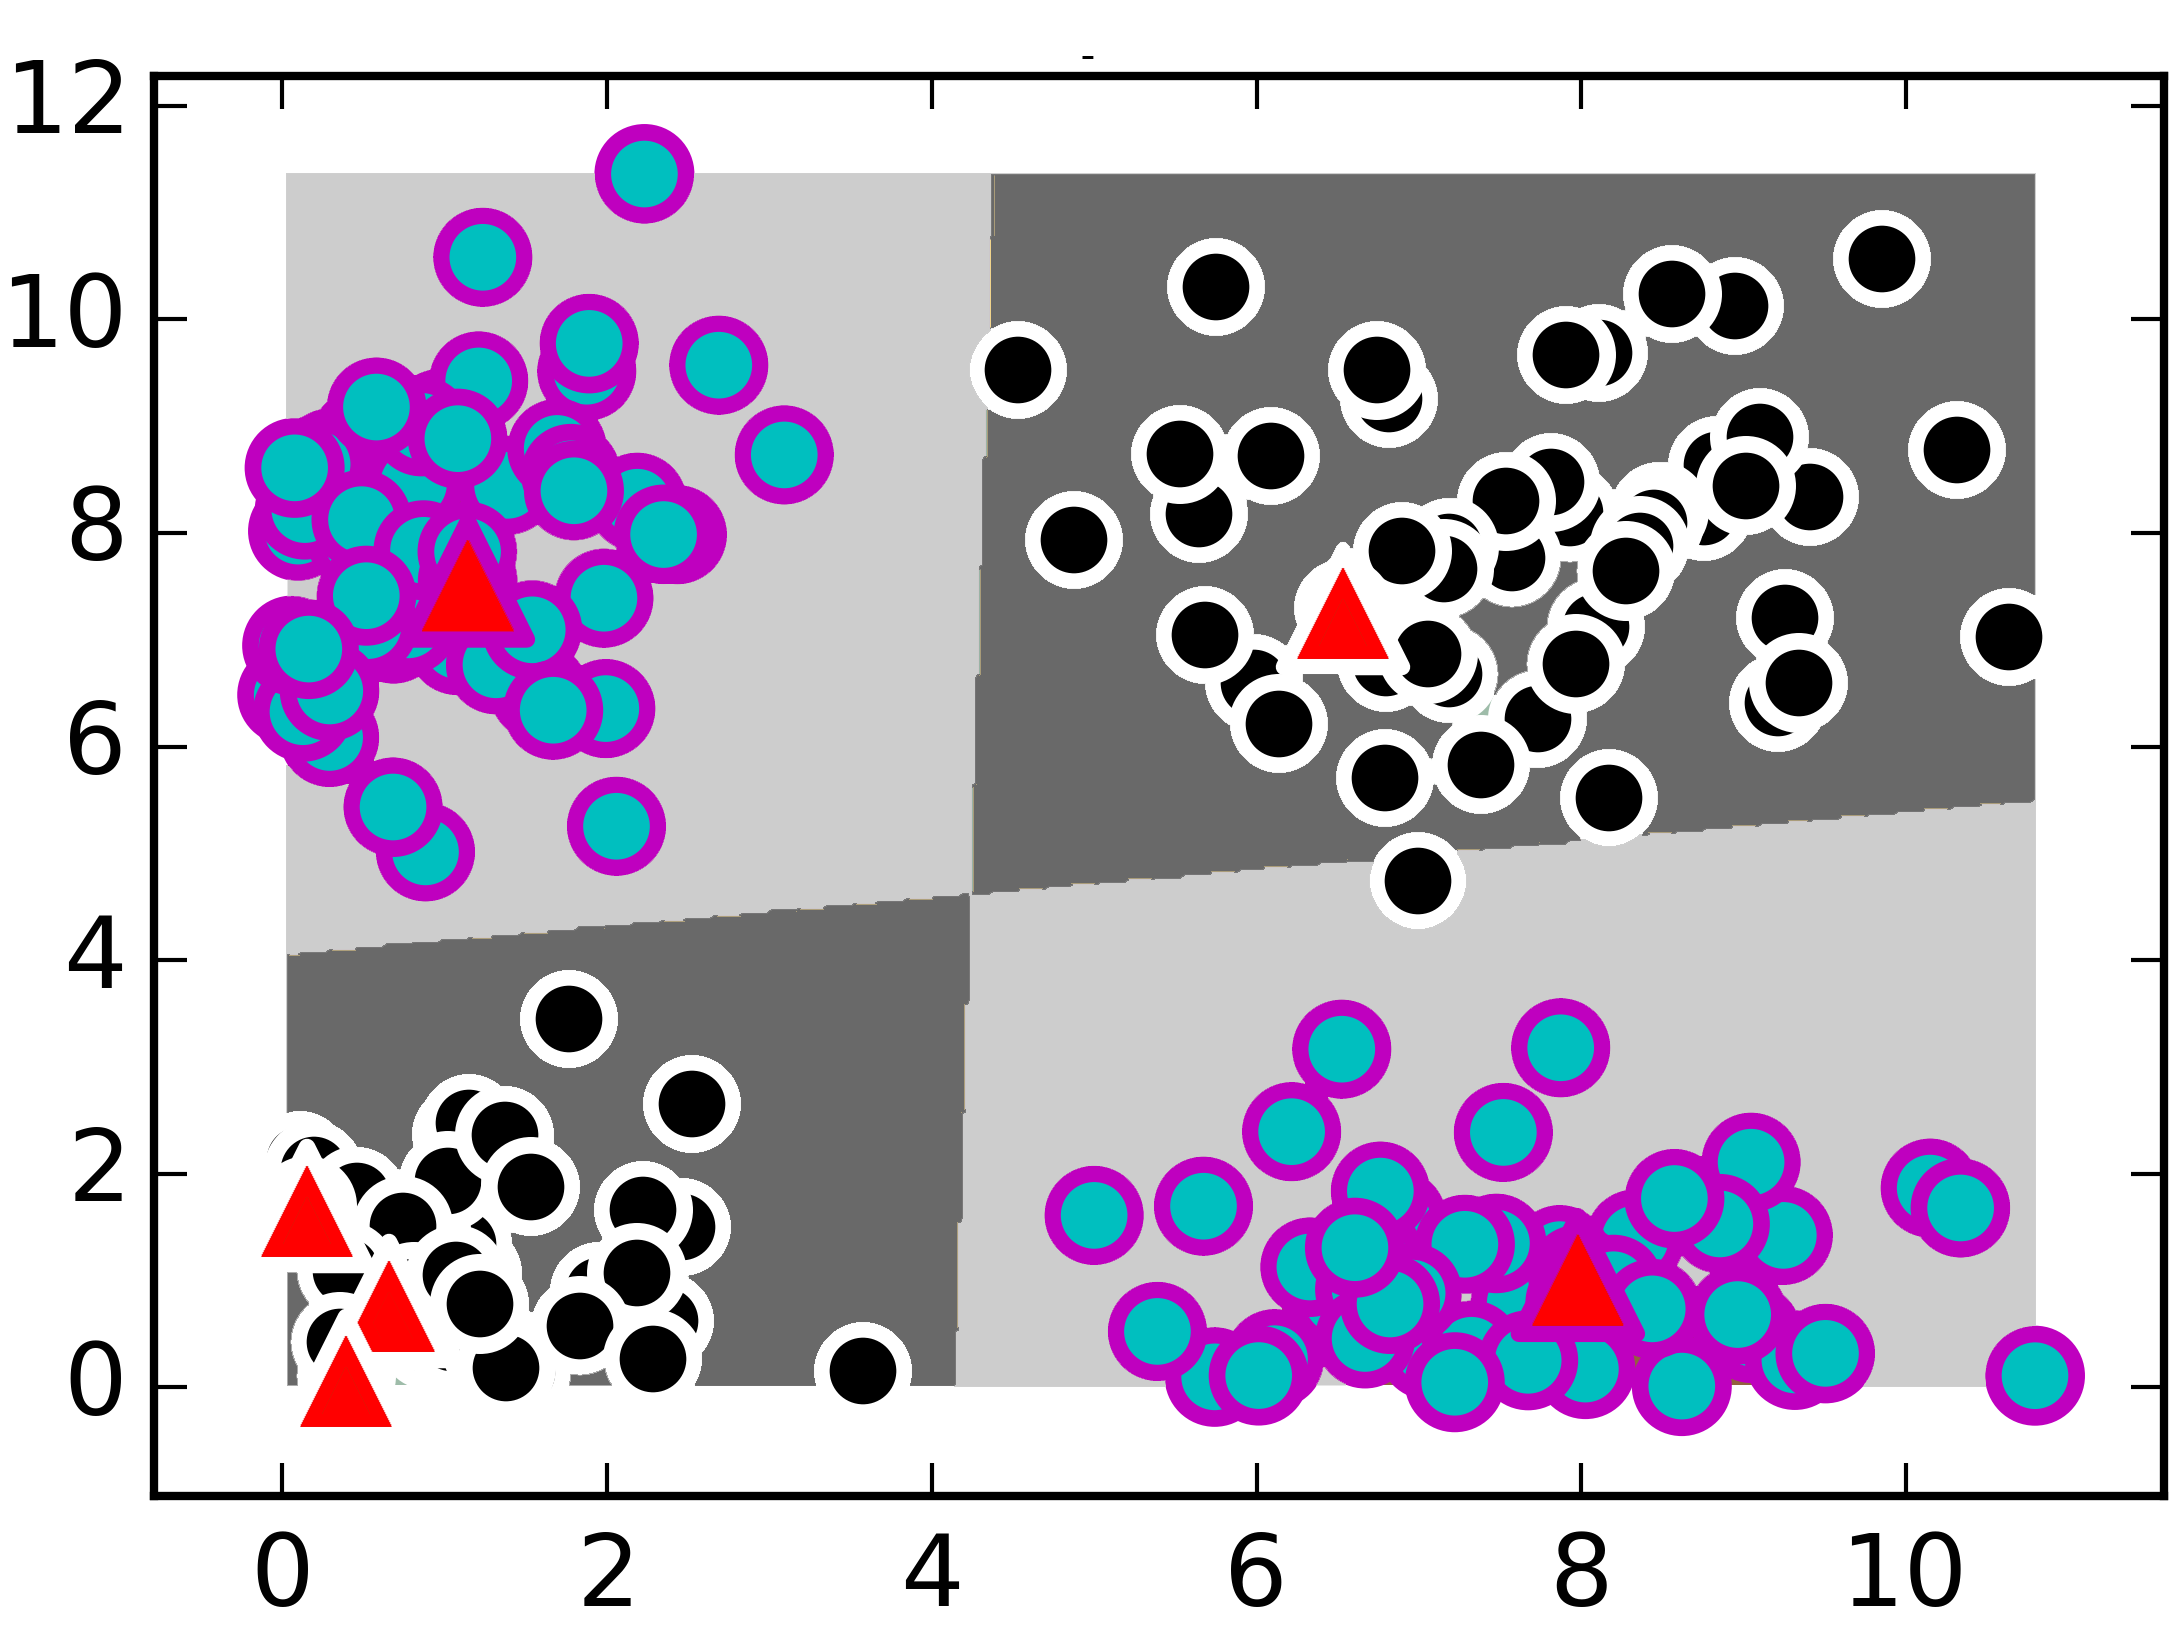
\includegraphics[width=0.25\textwidth]{quadplot2}%
	}
	\subfloat[Non-isotropic data]{%
		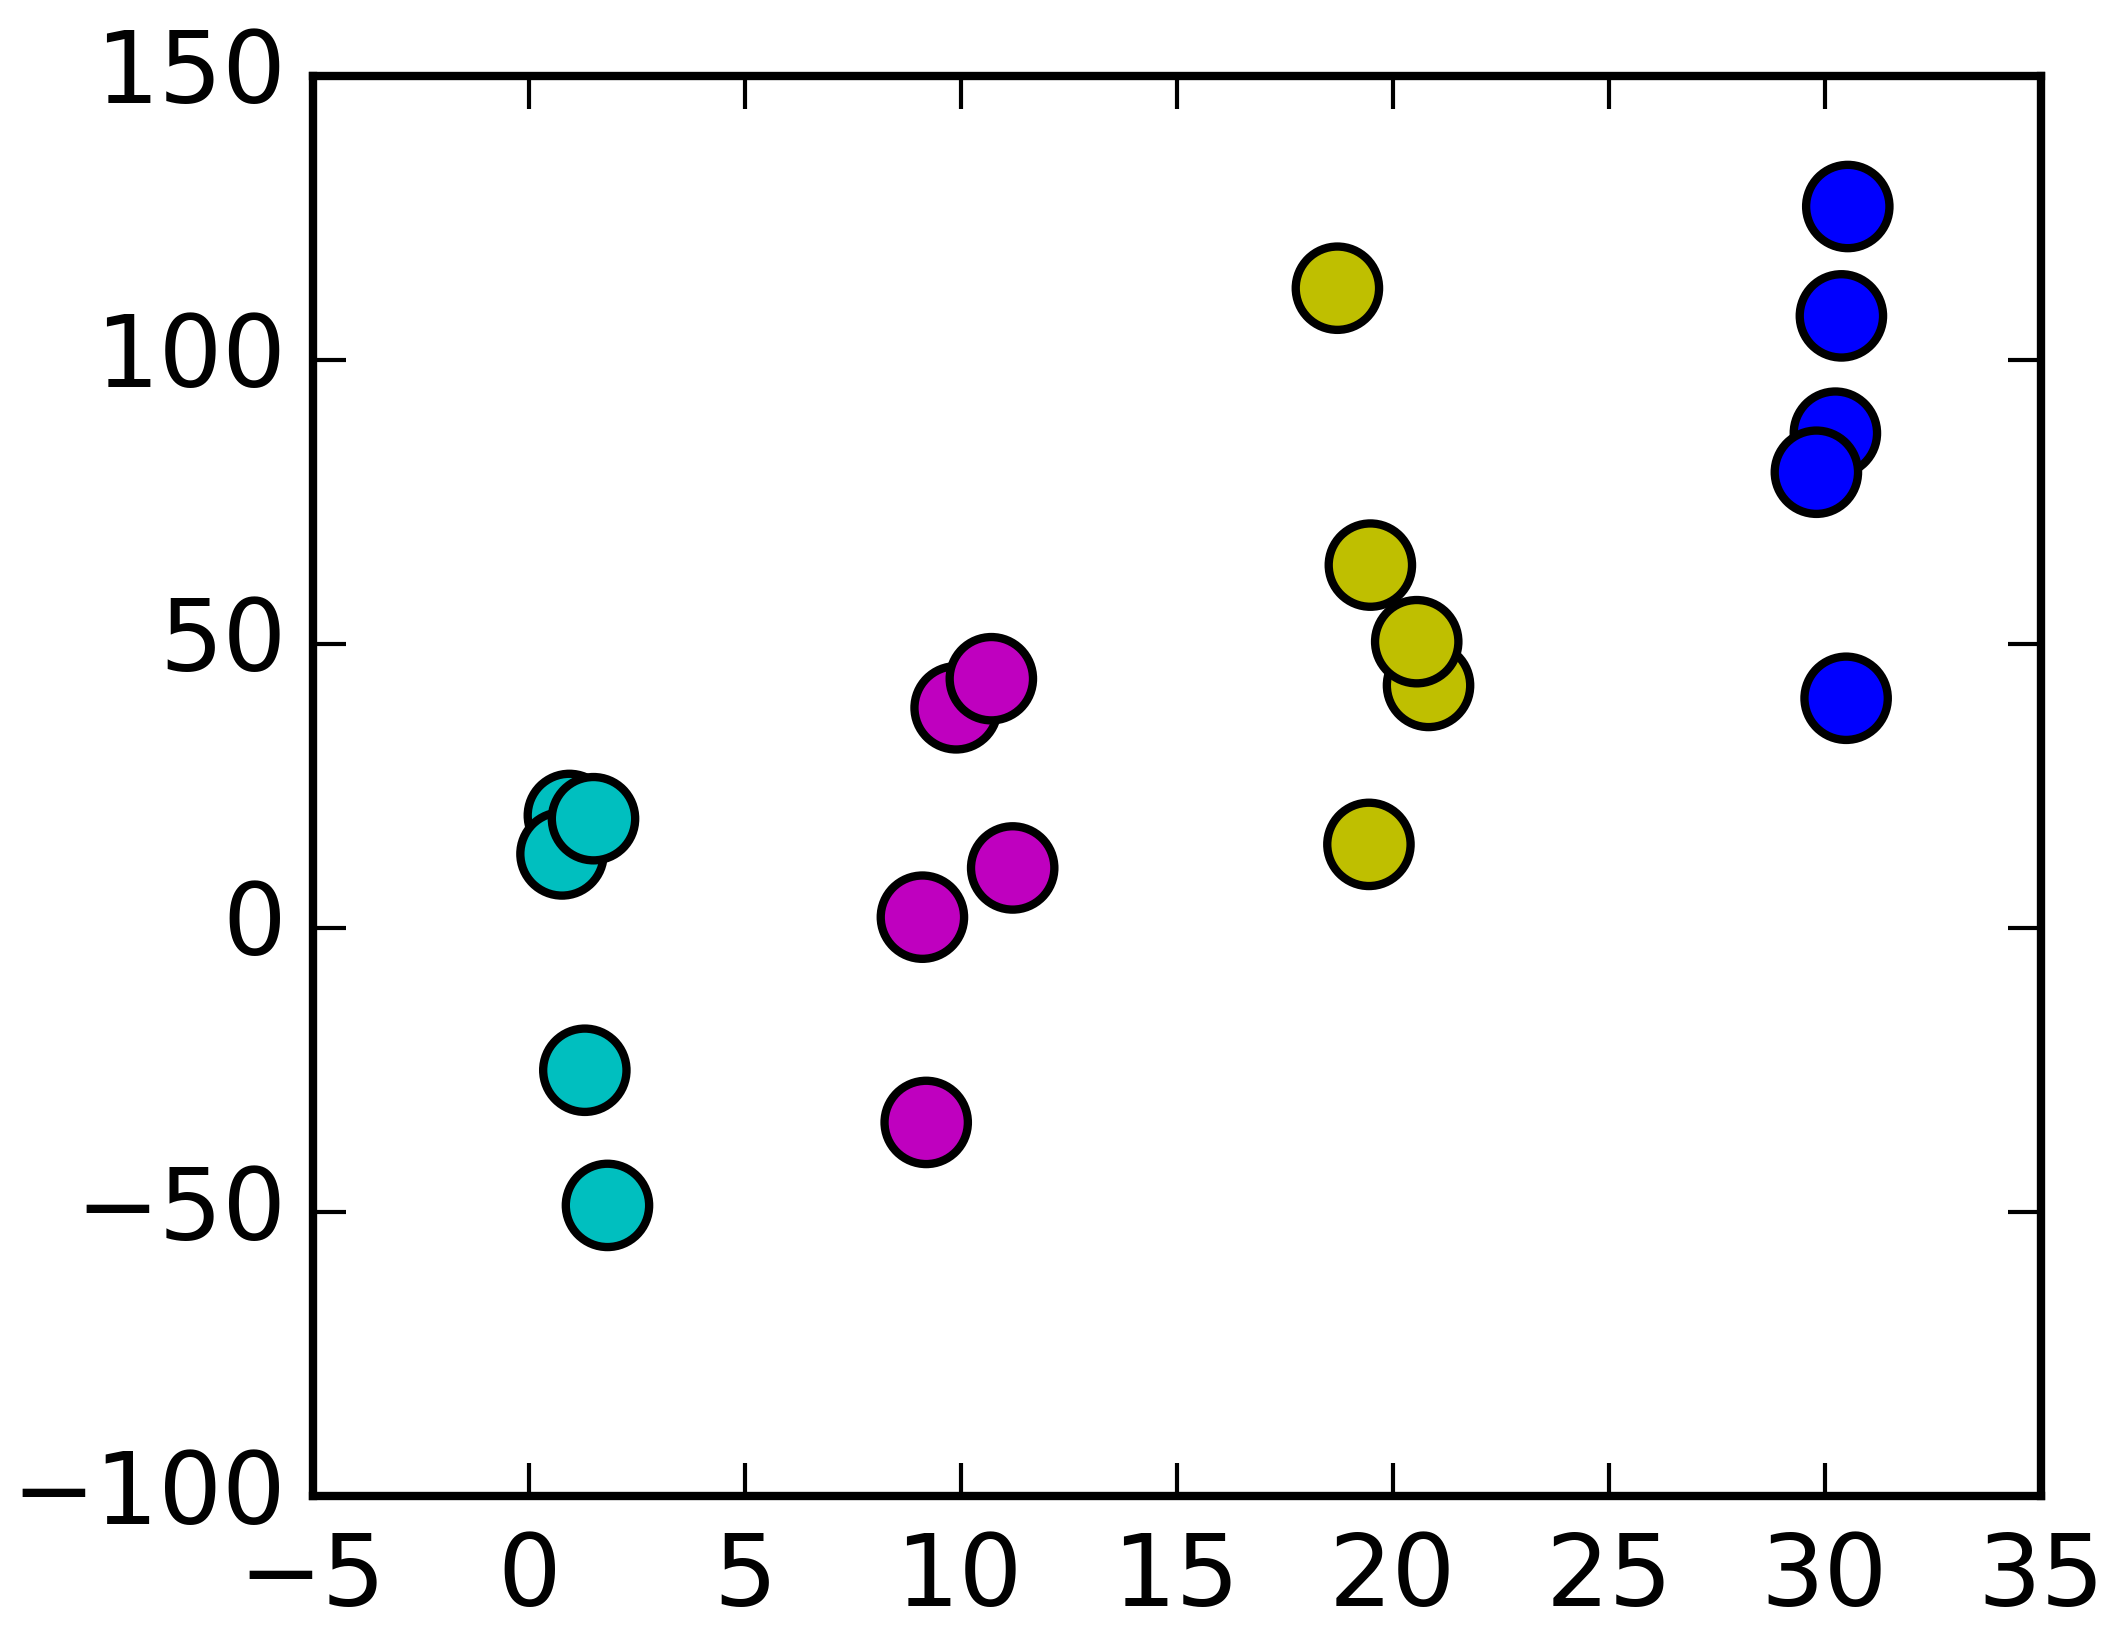
\includegraphics[width=0.25\textwidth]{isosvmproblem1}%
	}
	\subfloat[Pairwise differences]{%
		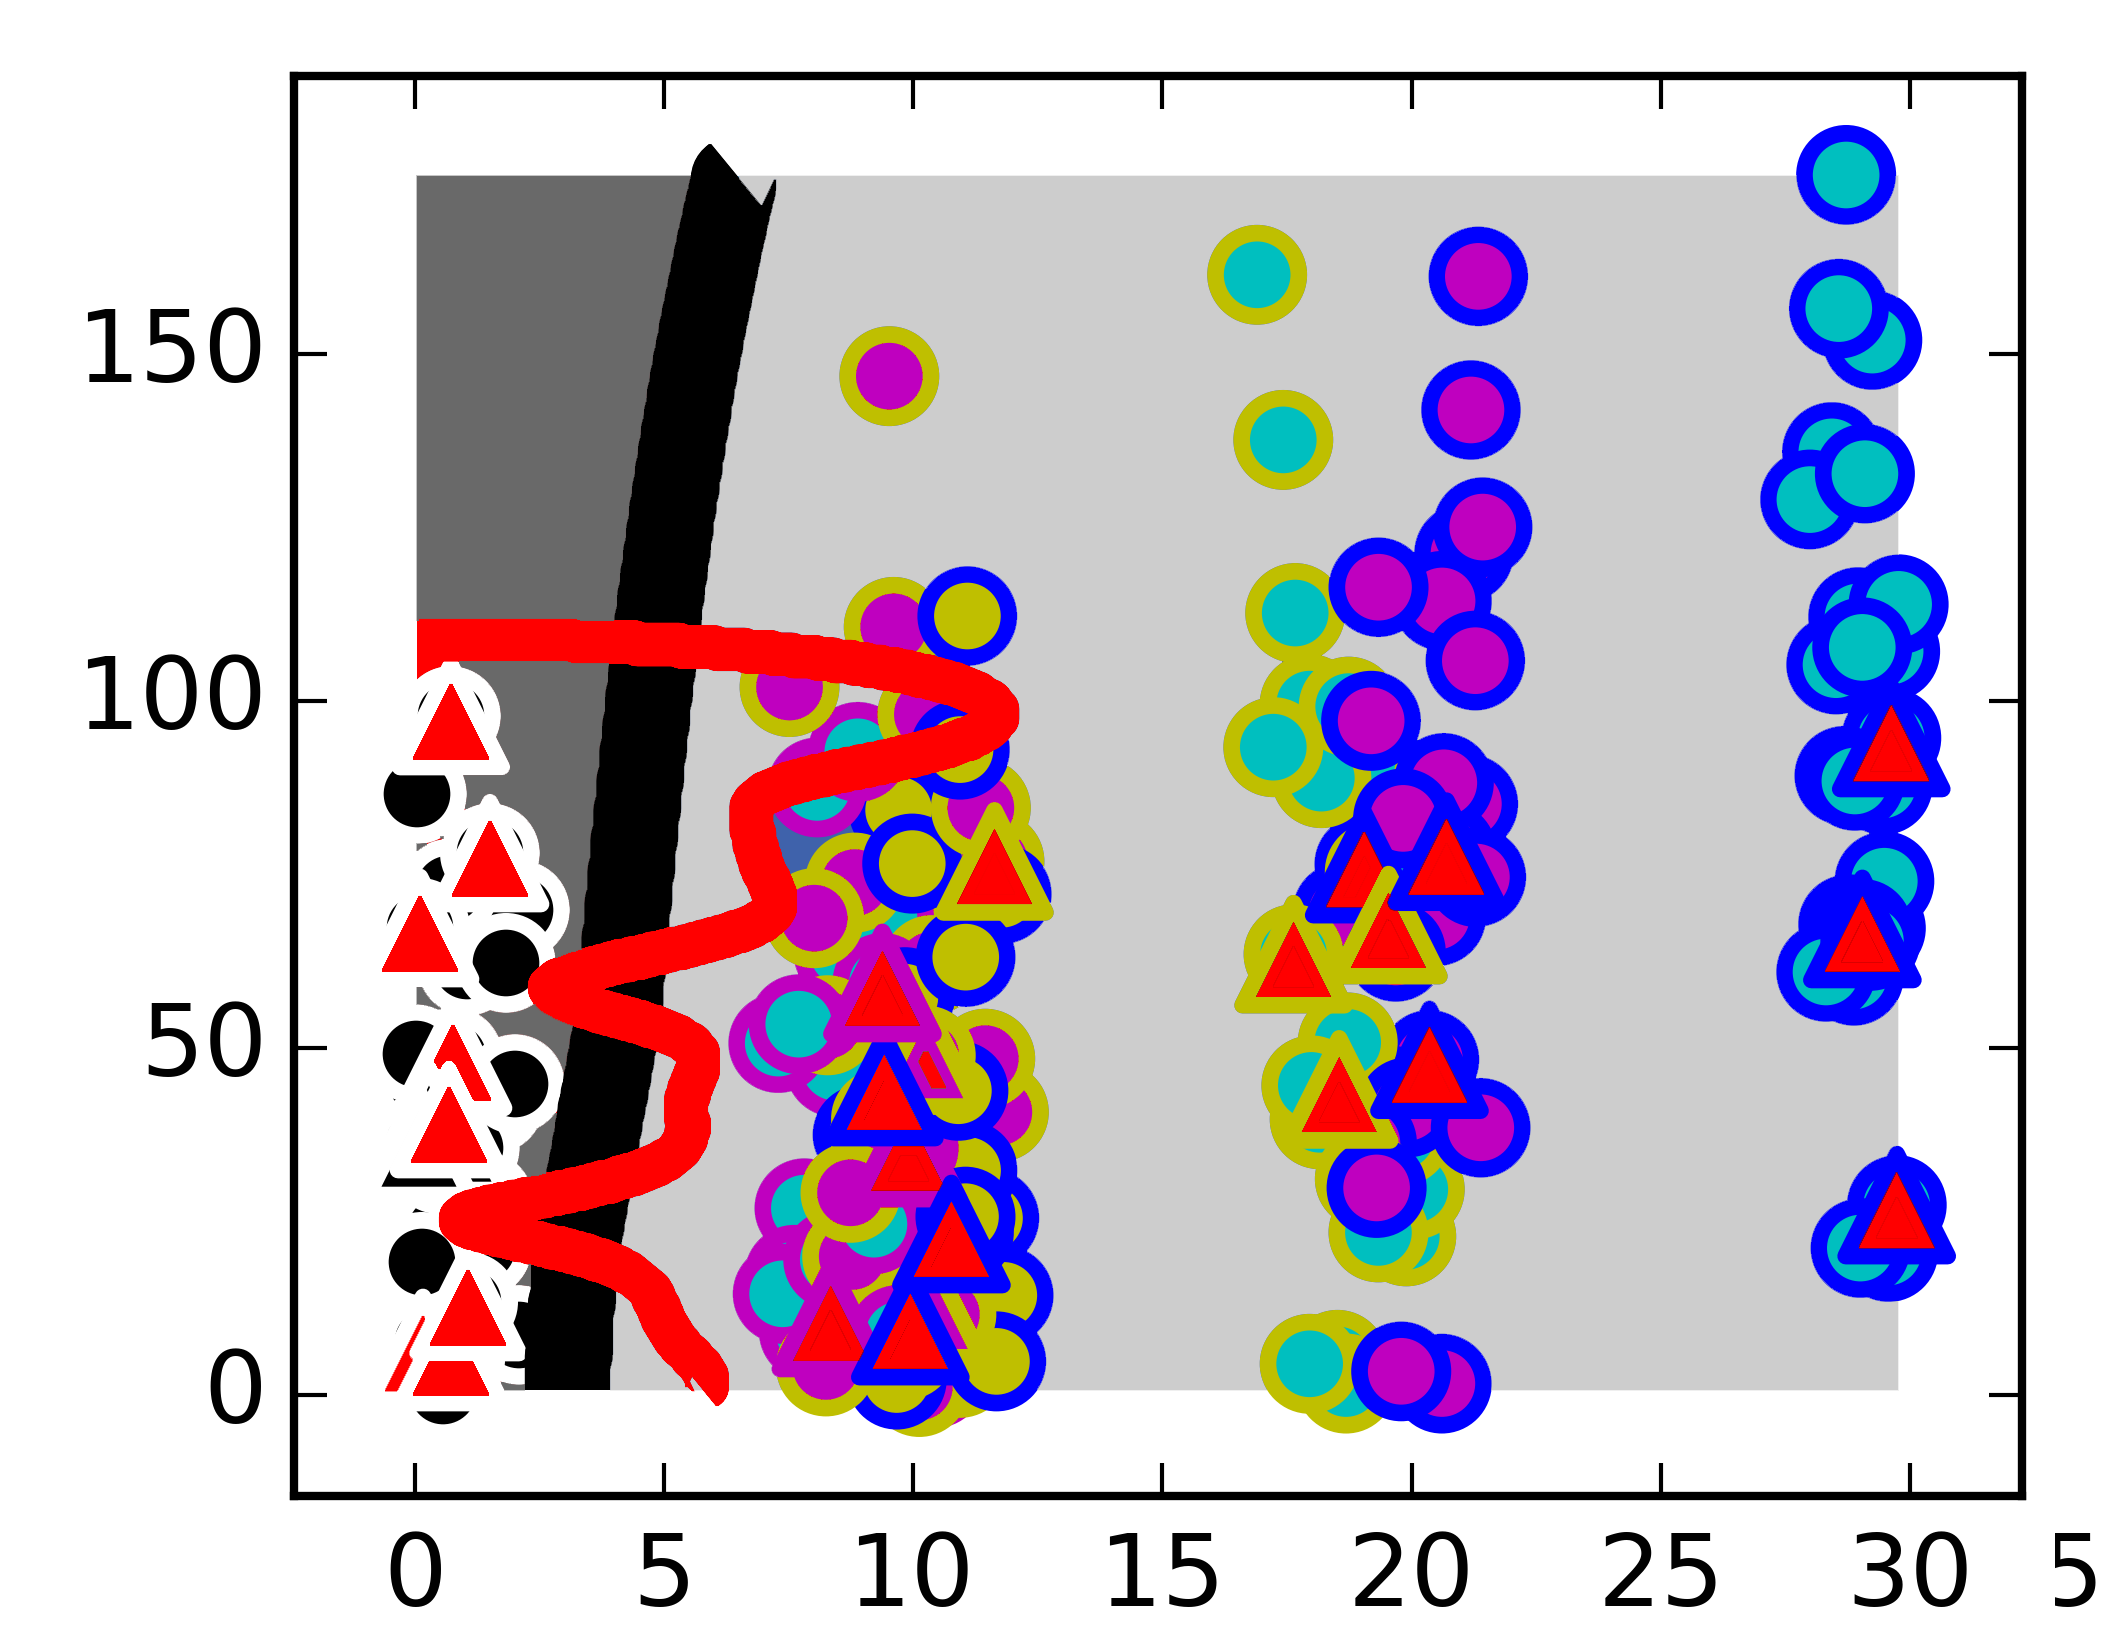
\includegraphics[width=0.25\textwidth]{isosvmproblem2}%
	}
	
	\caption[Motivation for the proposed metric learning approach]{Motivation for the proposed metric learning approach. (a) Example not linearly separable data requiring non-linear metrics. (b) Visualization of the distribution of corresponding absolute pairwise differences (APD), containing the element-wise differences in all dimensions between all possible objects, within (black) and across (coloured) clusters. The background contour shows the probability of a pair with a given distance belonging to the same cluster, learned by Gaussian Discriminant Analysis, and used as the distance pseudometric. Red triangles show the labelled constraints. (c) Example data with non-isotropic variance (three orders of magnitude larger in the y-axis direction). (d) Corresponding APD space coloured as in (a). In addition to the modelled probability of belonging to the same cluster, the models decision boundary (black), as well as the decision boundary of a Support Vector Machine with an isotropic RBF kernel (optimal parameters set by grid search), which overfits along the low-variance dimension.}
	\label{fig:motivation2}
\end{figure*}
 
In contrast, our method sidesteps the difficulty of robustly finding a good non-linear metric for a particular dataset, in a probabilistic framework, without hyperparameter tuning (it has a closed form solution and estimates all parameters from the data). Furthermore, instead of learning a metric using an objective function based on Lp-distance, which collapses the differences along the individual dimensions into one value, it lets the model directly access these individual differences, and thus to learn their importance, allowing it to easily deal with non-isotropic data (Figure \ref{fig:motivation2}c-d). 

Third, it makes explicit the structure in the distribution of constraints. It has been observed before that for data containing clusters, the probability density function of pairwise Lp distances shows two peaks (one for within- and one for across-cluster pairs), e.g. by \citep{brin1995near}. However, in the case of multiple clusters with different shapes and variances, a bimodal distribution is insufficient to reflect the true distributions of the instance differences within or across clusters. Clearly, within-cluster variances in one cluster do not have to equal those in another cluster, and the same is true for across-cluster variances (as illustrated by the variances of the groups of data in APD space in Figure \ref{fig:motivation2}b and d). Learning in pairwise difference vector space (instead of collapsing these distances into scalars) allows our model to adapt locally to within- and across-cluster variances of different clusters, and therefore to better approximate the true pairwise distance distribution. 

\section{Preliminary results}

We use Gaussian Discriminant Analysis (GDA) to learn a data distribution in APD space, and then use this model as a distance function with which to perform clustering, as used to model human spatial representation structure in Chapter 5 (however, note that any probabilistic model could be used in the metric framework introduced in Equation \ref{eq:metric} in Chapters 2.5, not just GDA). To show that the model is not only applicable to human spatial representation data, but also in other domains, we show clustering performance against 5 benchmark datasets used by \citep{zeng2012semi}, and compare it against a recent constrained clustering approach, Constrained Maximum Margin Clustering (CMCC) \citep{zeng2012semi}. 

We evaluate different approaches to perform clustering with the learned distance metric, including the Gaussian Mixture Model (similar to the DP-GMM, but given the correct number of clusters), spectral clustering \citep{ng2002spectral}, weighted, complete, average and Ward agglomerative clustering \citep{mullner2013fastcluster}, and the well-known K-Means clustering algorithm \citep{hartigan1979algorithm}. Figure \ref{mlclust} shows the results.


\begin{figure*}[t]
	\centering
	
	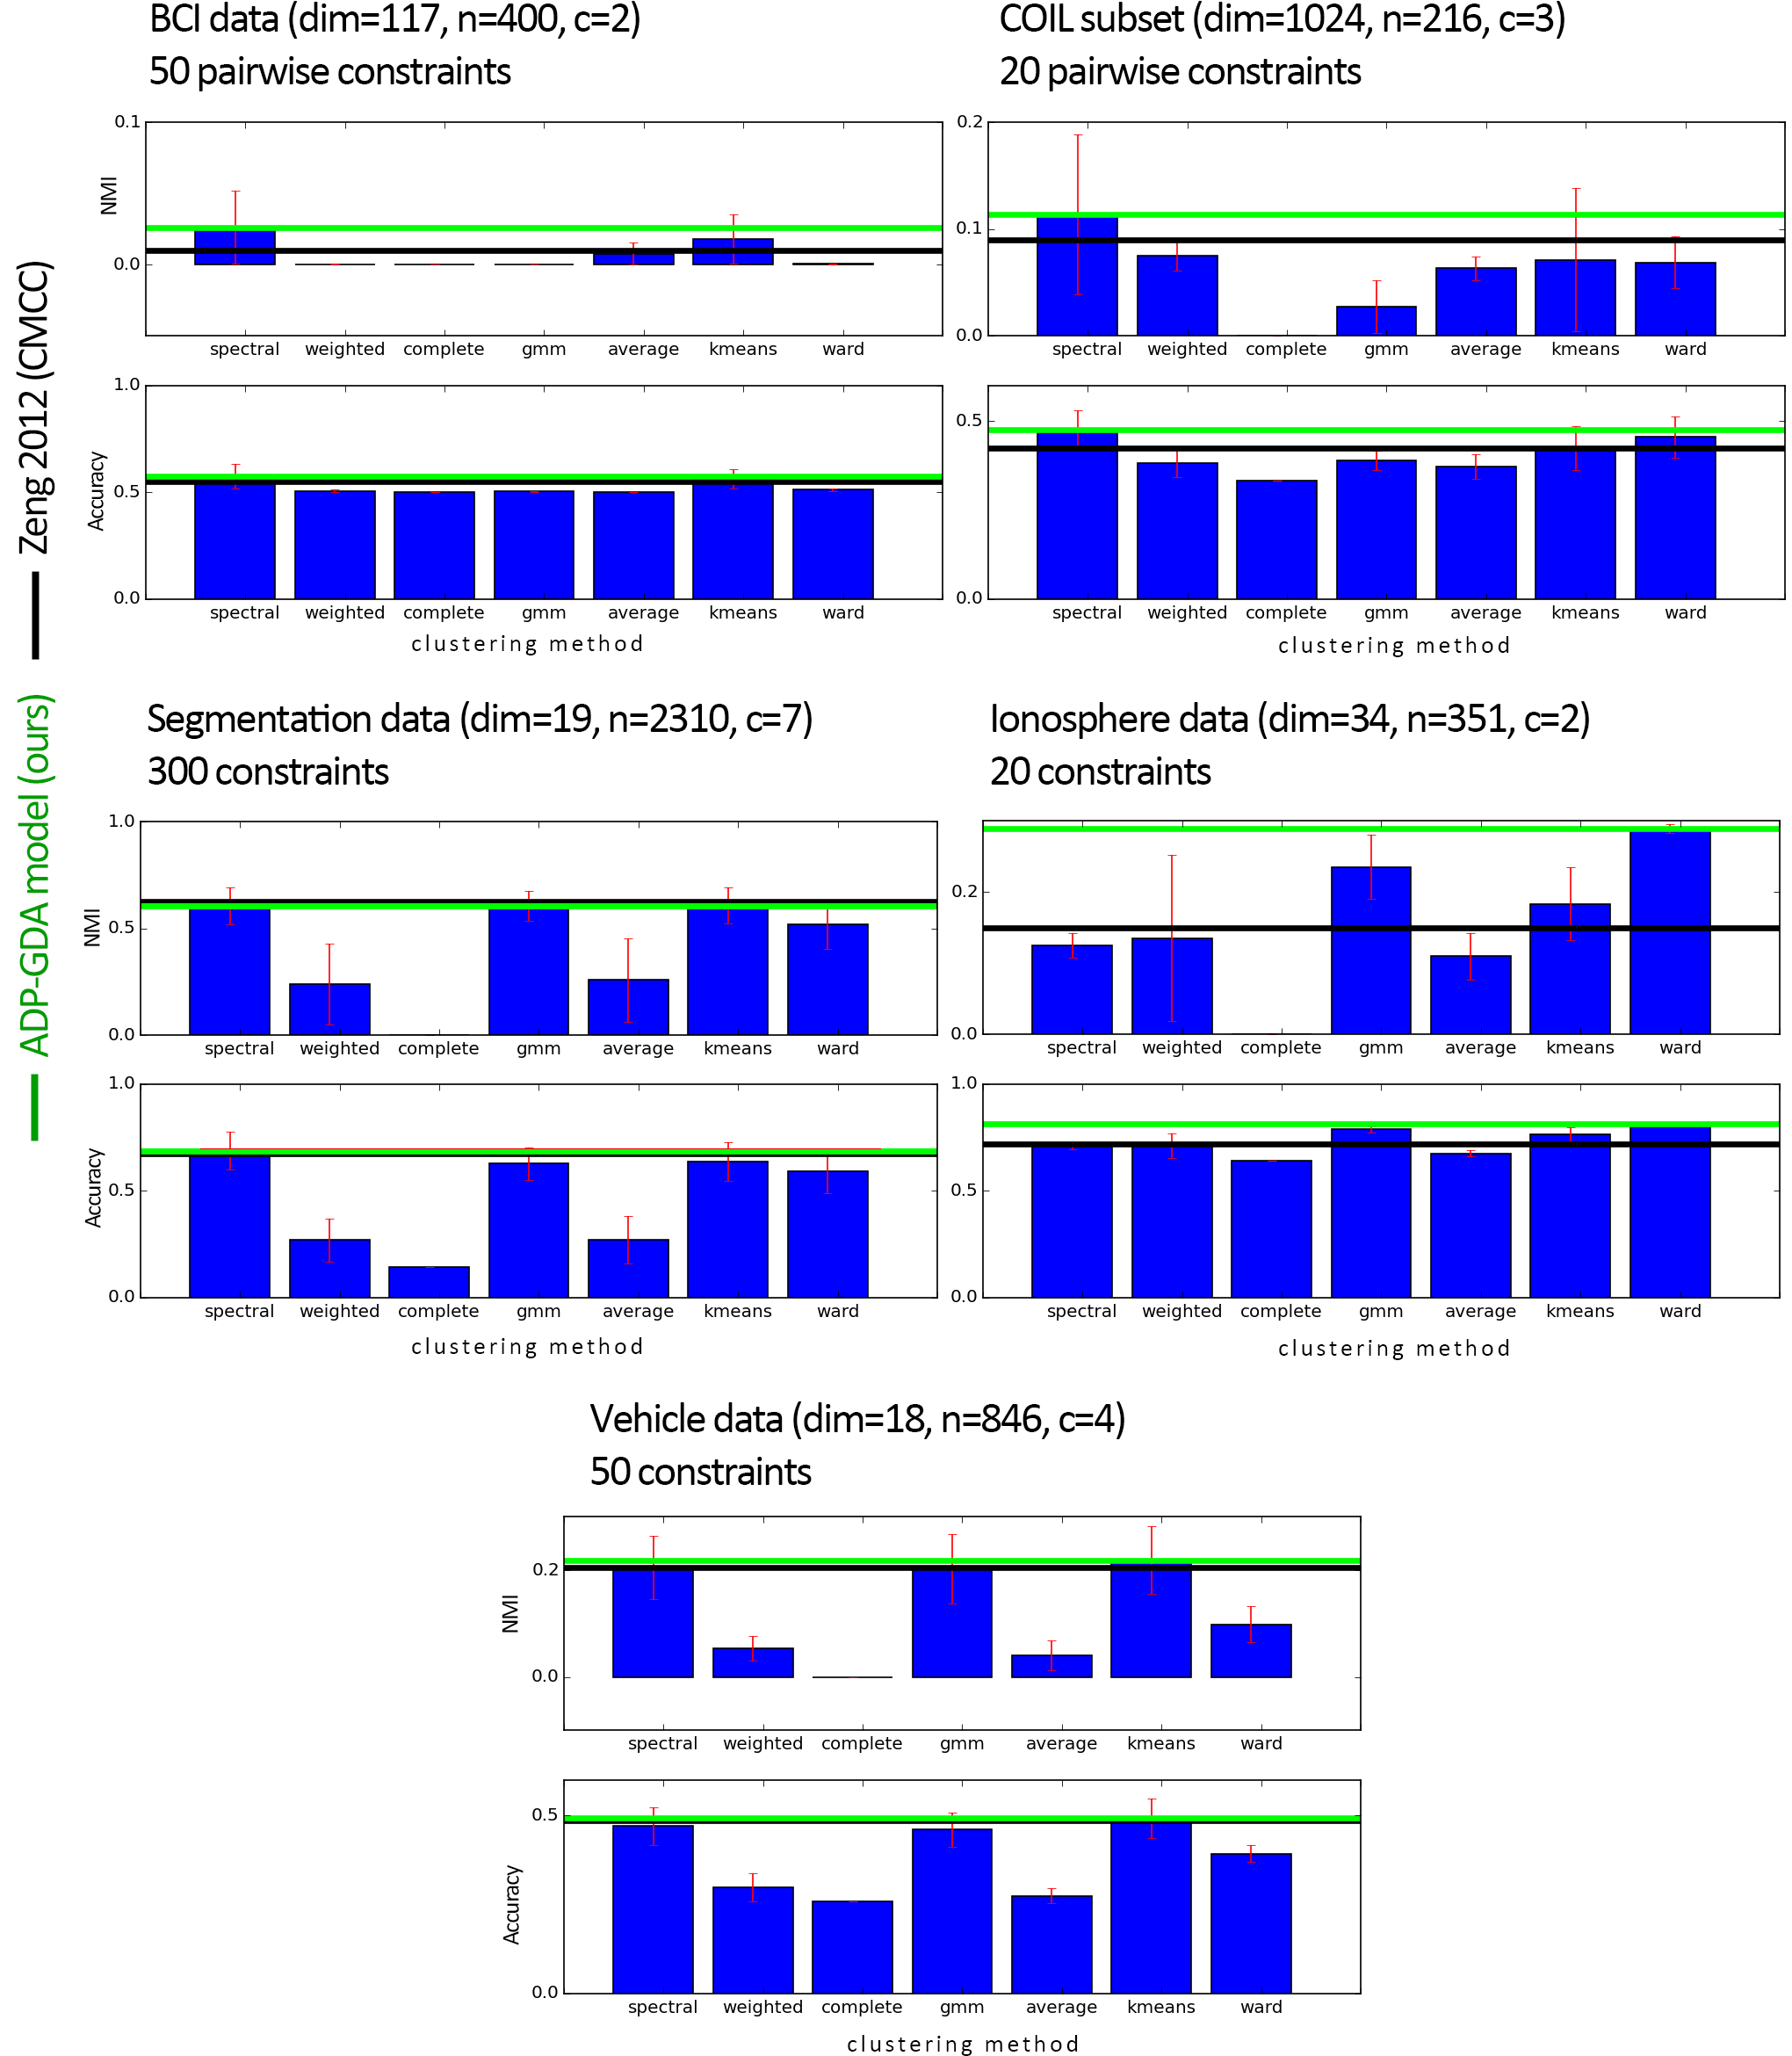
\includegraphics[width=\textwidth]{adsgda_mlresults}%
	
	\caption[Clustering results using the ADS-GDA metric on benchmark datasets]{\textbf{Clustering results using the ADS-GDA metric on benchmark datasets}. Evaluation metrics: NMI (normalized mutual information) and Accuracy (percentage of correctly assigned data points). Abbreviations: dim...dimensionality, n...number of data points, c...clusters.}
	\label{mlclust} 
\end{figure*}


